\documentclass[conference]{IEEEtran}
\IEEEoverridecommandlockouts
% The preceding line is only needed to identify funding in the first footnote. If that is unneeded, please comment it out.
\usepackage{cite}
\usepackage{amsmath,amssymb,amsfonts}
\usepackage{algorithmic}
\usepackage{graphicx}
\usepackage{textcomp}
\usepackage{xcolor}
\def\BibTeX{{\rm B\kern-.05em{\sc i\kern-.025em b}\kern-.08em
    T\kern-.1667em\lower.7ex\hbox{E}\kern-.125emX}}


\usepackage{graphicx}
\usepackage{multicol}
% para el codigo fuente
\usepackage{listings}
\usepackage{color}
\definecolor{dkgreen}{rgb}{0,0.6,0}
\definecolor{gray}{rgb}{0.5,0.5,0.5}
\definecolor{mauve}{rgb}{0.58,0,0.82}
\lstset{frame=tb,
	language=Python,
	aboveskip=3mm,
	belowskip=3mm,
	showstringspaces=false,
	columns=flexible,
	basicstyle={\small\ttfamily},
	numbers=none,
	numberstyle=\tiny\color{gray},
	keywordstyle=\color{blue},
	commentstyle=\color{dkgreen},
	stringstyle=\color{mauve},
	breaklines=true,
	breakatwhitespace=true,
	tabsize=3
}

\usepackage[spanish]{babel}

\renewcommand{\figurename}{Figura.}
\renewcommand{\tablename}{Tabla.}
\renewcommand{\abstractname}{Resumen}

\begin{document}

\title{Implementación de la tesis: \\``Multiple Sequence Alignment using Particle Swarm Optimization''}

\author{\IEEEauthorblockN{1\textsuperscript{st} Vicente Machaca Arceda}
\IEEEauthorblockA{\textit{DAISI} \\
\textit{Universidad Nacional de San Agustín}\\
Arequipa, Perú \\
vmachacaa@unsa.edu.pe}

}

\maketitle

\begin{abstract}
Este reporte presenta la implementación y análisis de la tesis: ``\textit{Multiple Sequence Alignment using Particle Swarm Optimization}''. Dicha tesis propone el uso de \textit{Particle Swarn Optimization} (PSO) para solucionar el problema de \textit{Multiple Sequence Alignment} (MSA). El autor propone la posición de cada \textit{gap}, como vector para la representación de las partículas, luego define un \textit{crossover} para simular el movimiento de una partícula hacia la partícula lider. Además, tambien se propone una mutación para diversificar la solución. En las pruebas realizadas, se comprobo que PSO obtiene muy buenos resultados e incluso similares a CLUSTALW.
\\
\end{abstract}

\begin{IEEEkeywords}
PSO, MSA, alineamiento de secuencias.
\end{IEEEkeywords}

\section{Introducción}
El area de Bioinformática ha tenido un auge en las ultimas decadas. Por ejemplo, el proyecto: \textit{The Human Genome Project} (HGP) que inicio en 1990 y fue completado el 2003, donde participarón varios paises como EEUU, Reino Unido, Japón, Francia, Alemania, España y China  \cite{hgp2021}; el proyecto tenia como objetivo secuenciar todo el genoma humano, el cual resulto ser una secuencia de aproximadamente 3.2 billones de pares de bases \cite{archibald2018genomics}. En la actualidad exixten diversas areas de investigación como: la prediccón de estructura de proteinas, predicción de la función de una proteina a partir de estructuras de redes de proteinas, descubrimiento de medicamentos, predicción de enfermedades a partir del genoma, análisis de virus, etc. Es tan grande este campo de estudio que incluso se ha dividido en otras areas como \textit{metagenomics}, \textit{proteomics}, \textit{chemical informatics}, etc. 

\subsection{Problema}

Uno de los tantos problemas que existen en bioinformática, es el alineamiento multiple de secuencias. Se puede definir el alineamiento de secuencias como un método que permite determinar el grado de similitud entre dos o más secuencias \cite{xiong2006essential}, además el método puede insertar \textit{gaps} dentro de las secuencias de consulta, con el objetivo de lograr la mayor cantidad de bases alineadas. Por ejemplo, en la Figura \ref{fig:msa}, se muestra el resultado luego de alinear varias secuencias de aminoacidos. Como podemos ver, se ha isertado \textit{gaps} (-) para así maximizar la cantidad de aminoacidos que coinciden en la misma posición. \\

\begin{figure*}[h]
	\centering
	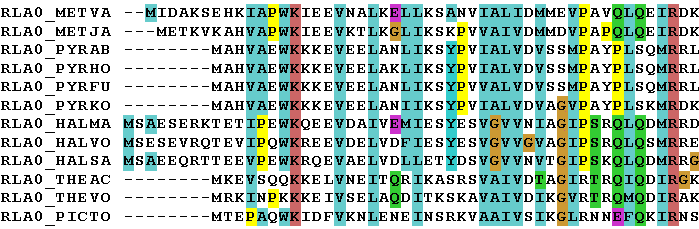
\includegraphics[width=0.6\textwidth]{images/msa}
	\caption{Ejemplo de \textit{Multiple Sequence Alignment} (MSA). El método ha insertado \textit{gaps} (-) en las secuecnias necesarias para maximizar la cantidad de letras (aminoacidos) que concidan en la misma posición.}
	\label{fig:msa}
\end{figure*}

El alineamiento de secuencias puede dividirse en dos grupos: \textit{pair-wise sequence alignment} (PSA) y \textit{multiple sequence alignment} (MSA) \cite{xiong2006essential}. La diferencia radica en que el primero alinea solo dos secuencias y el segundo puede alinear dos a mas secuencias. Además, el problema de MSA es considerado un problema NP completo \cite{wang1994complexity}. Debido a esto es que se han planteado heuristicas que logran obtener una solución local; el algoritmo mas utilizado es CLUSTAL, fue propuesto por \cite{higgins1988clustal}, este algoritmo ha sido mejorado con CLUSTALV \cite{higgins1992clustal}, CLUSTALW \cite{thompson1994clustal} y CLUSTALX \cite{jeanmougin1998multiple}. Otro algoritmo importante es MUSCLE \cite{edgar2004muscle}. \\


El problema de los algoritmos mencionados anteriormente, es que a pesar de ser heurísticas, el tiempo de procesamiento es muy alto. Cada segundo los datos genómicos crecen exponencialmente \cite{archibald2018genomics} y los algoritmos utilizados para buscar información en estas bases de datos, son basados en alineamiento. Entonces, mientras mas crecen los datos, mas lentos se vuelven estos algoritmos \cite{zablocki2009multiple}. 

\subsection{Objetivo}

El autor propone en su tesis aplicar \textit{Particle Swarm Optimization} (PSO) como alternativa a CLUSTAL para solucionar el problema de MSA.\\


\section{Conceptos básicos}

\textbf{Secuencia de ADN y aminoacidos}: Si hablamos de ADN, nos referimos al conjunto de bases nitrogenadas Adenina (A), Citosina (C), Guanina (G) y Timina (T). Pero si nos referimos a aminoacidos, estos son 20 y son representados con letras desde la A hasta la V \cite{xiong2006essential}. \\

\textbf{Secuenciamiento de ADN}: Proceso por el cúal se determina el orden de cada base (A, T, C y G) presente en el genoma \cite{archibald2018genomics}.\\

\textbf{Alineamiento de secuencias}: Proceso por el cúal se comparan dos o más secuencias de ADN para determinar su grado de similitud \cite{xiong2006essential}. Existen dos tipos: \textit{pair-wise sequence alignment}, donde se alinean dos secuancias y \textit{Multiple Sequence Alignment} (MSA), cuando alineamos mas de dos secuencias. Los algoritmos mas utilizados son: BLAST y CLUSTAL.\\ 

\textbf{Gap}: Caracter ``-'' insertado durante el alineamiento de secuencias para alinear cada base y maximizar el grado de similitud.\\



\section{Trabajos relacionados}


El algoritmo mas utilizado para alinear dos secuencias de ADN o aminoacidos es BLAST \cite{altschul1997gapped}. Este método a tenido varias mejoras como TurboBLAST \cite{bjornson2002turboblast},  ScalaBLAST \cite{oehmen2006scalablast}, Usearch \cite{edgar2010search} y  ScalaBLAST 2.0 \cite{oehmen2013scalablast}. Pero si hablamos de alinear mas de dos secuencias, el algoritmo mas utilizado es  CLUSTAL \cite{higgins1988clustal}, con mejoras en CLUSTALV \cite{higgins1992clustal}, CLUSTALW \cite{thompson1994clustal} y CLUSTALX \cite{jeanmougin1998multiple}.  \\


El problema de MSA, tambien ha sido tratado de solucionarse con métodos \textit{alignment-free}. Uno de los primeros métodos fue propuesto por Xu \cite{xu2009method} y Zhang \cite{hongwei2005pso}. Pero, recientemente, se ha propuesto PSO en dos niveles \cite{lalwani2017efficient, lalwani2019efficient}. Tambien, se ha presentado una versión llamada \textit{chaotic-PSO} \cite{lei2009multiple} y otras versiones híbridas \cite{rasmussen2003improved, chaabane2018hybrid}. 

\section{Metodología aplicada}

En esta sección describimos la metodología planteada por el autor para solucionar el problema de MSA utilizando PSO.

\subsection{Representación de las partículas}

Un de los primeros pasos para solucionar un problema utilizando PSO, es la representación de cada particula. El autor propone utilizar la posición de cada \textit{gap} como un vector. Por ejemplo en al Figura \ref{fig:pso_1}, tenemos la representación del la partícula \textit{leader} y una partícula cualquiera (ambas representan una posible solución al problema). Ahora en la Figura  \ref{fig:pso_2}, tenemos otra forma de representar dichas partículas, en este caso solo estamos considerando la posición de cada \textit{gap} insertado. La opción mas facil de controlar es la correspondiente a la Figura \ref{fig:pso_2}. \\

\begin{figure}[h]
	\centering
	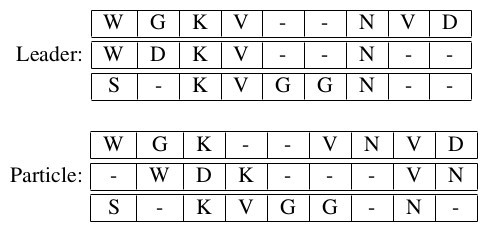
\includegraphics[width=0.4\textwidth]{images/pso_1}
	\caption{Ejemplo de la partícula \textit{leader} y una partícula cualquiera. Ambas representan una posible solución a un problema de alineamiento de 3 secuencias de aminoacidos.}
	\label{fig:pso_1}
\end{figure}

\begin{figure}[h]
	\centering
	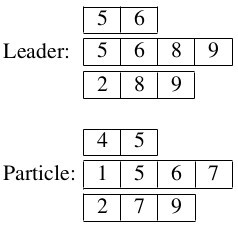
\includegraphics[width=0.2\textwidth]{images/pso_2}
	\caption{Ejemplo de la partícula \textit{leader} y una partícula cualquiera. En este caso solo estamos registrando la posición de cada \textit{gap } insertado.}
	\label{fig:pso_2}
\end{figure}

\subsection{Movimiento de las partículas}
Según el algoritmo de PSO, cada partícula debe acercarse al \textit{leader} en cada iteración. Este acercamiento será implementado haciendo un \textit{crossover}. El \textit{crossover} permitirá que la nueva partícula (partícula en movimiento) tenga información de ambas partículas (\textit{leader} y la partícula en movimiento).  \\

Para aplicar un \textit{crossover} entre dos partículas, debemos calcular primero la distancia entre ellas aplicando la formula de la Ecuación \ref{eq:distance}. Luego debemos calcular el punto de cruce de ambas partículas, para esto aplicamos la formula de la Ecuación \ref{eq:crosspoint}, en este caso $length$ representa la longitud de las secuencias.\\



\begin{equation}\label{eq:distance}
distance =  \dfrac{ matchingGaps }{totalGaps} 
\end{equation}

\begin{equation}\label{eq:crosspoint}
crossPoint =  rand( 1, distance*length )
\end{equation}

Por ejemplo, dada las partículas de la Figura \ref{fig:pso_2} y suponiendo que hemos obtenido un \textit{crossPoint = 5},  utilizando la Ecuación \ref{eq:crosspoint}. La partícula en movimiento se desplazaría y su nueva representación sería el resultado de aplicar un \textit{crossover}. En la Figura \ref{fig:pso_3} mostramos el resultado de aplicar el \textit{crossover}. Para lograr esto, por cada secuencia del leader insertamos sus gaps en la nueva partícula que son menores o iguales al $crossPoint$, luego completamos insertando los \textit{gaps} de la partícula en movimiento que tengan \textit{gaps} mayores al $crossPoint$.



\begin{figure}[h]
	\centering
	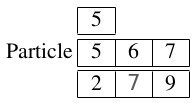
\includegraphics[width=0.17\textwidth]{images/pso_3}
	\caption{Resultado del movimiento de una partícula luego de aplicar \textit{crossover}.}
	\label{fig:pso_3}
\end{figure}


\subsection{Función objetivo}
La función objetivo propuesta, es la misma utilizada para medir el desempeño de los algoritmos basados en alineamiento como CLUSTAL para el problema de MSA. Por ejemplo en la Figura \ref{fig:fo}, se presenta un ejemplo del cálculo del \textit{score} del alineamiento de dos secuencias. En este ejemplo se utilizo un  \textit{match score} : +1, \textit{mismatch score}: 0, \textit{openning gap}: -1 y \textit{gap penalty}: -1. Para el caso de MSA, se procesa este \textit{score} por cada posible conbinación de dos secuencias. Para los experimentos se usaron estos mismos valores.

\begin{figure}[h]
	\centering
	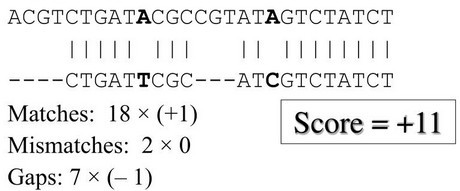
\includegraphics[width=0.3\textwidth]{images/fo}
	\caption{Ejemplo del cálculo del \textit{score} del alineamiento de dos secuencias de ADN. En este caso se utilizo: \textit{match score} : +1, \textit{mismatch score}: 0, \textit{openning gap}: -1 y \textit{gap penalty}: -1}
	\label{fig:fo}
\end{figure}

\subsection{Mutaciones}
Para diversificar al algoritmo de PSO, Se propuso hacer mutaciones a las partículas. El proceso de mutación consistia en escoger de manera aleatoria una partícula, luego dentro de dicha partícula se escogia una secuencia y se insertaba un \textit{gap} en una posición aleatoria. Luego, para que todas las secuencias dentro de la partícula tengan la misma longitud, se insertaba un \textit{gap} al principio o al final según un valor generado aleatoriamente.


\section{Experimentos}

En esta sección detallaremos las bases de datos utilizadas y los parametros del algoritmo PSO para poder replicar los resultados.

\subsection{Bases de datos}
El autor propone un conjunto de 7 bases de datos. S1, S2, S3, S4, S5, S6 y S7 que el construyo a partir de un conjunto de secuencias de ADN. En la Tabla \ref{tab:datasets}, presentamos el \textit{ascension code} de cada secuencia utilizada. Ademas, el autor propuso un conjunto pequeño de secuencias para hacer pruebas rapidas, a este conjunto lo llamo S8. En nuestro caso, al ser una tesis un poco antigua, algunas secuencias ya no estaban disponibles en NCBI, y solo logramos obtener las secuencias de S6, S7 y S8. \\

\begin{table}[h]
	\caption{Bases de datos utilizados por \cite{zablocki2009multiple}. S1, S2, S3, S4, S5, S6 y S7 es el nombre que el autor definio para cada conjunto de secuencias. La segunda columna representa el \textit{ascension code} de cada secuencia.}
	\begin{tabular}{lp{7cm}}
		
		\textbf{\textit{Dataset}} & \textbf{Secuencias} \\
		\hline			
		S1	& HCV2L1A10 HCV2L3A5 HCV2L3C1 HCV2L3C8 HCV2L3D4 HCV2L3E6 HCV2L3A7 HCV2L3A9 HCV2L3B2  HCV2L3B1		\\				
		S2	& HS06674 HS06675 HS06676 HS06677 HS06679 \\
		S3  & TPAHISIN TNIHISIN TNHISIN TMIHISIN TMHISIN THHISIN TFHISIN TEHISIN TCUHISIN TCHISIN TBHISIN TAUHISIN TAHISIN TTHISIN TSHISIN TRHISIN TPYHISIN TPIHISIN TPHISIN TCAHISIN TLHISIN \\
		S4  & HI1U16764 HI1U16766 HI1U16768 HI1U16776 HI1U16778 HI1U16770	HI1U16774	HI1U16772 \\
		S5  & HI1U16765 HI1U16767 HI1U16769 HI1U16771 HI1U16773	HI1U16775 HI1U16777 HI1U16779 \\
		S6  & PP59651 PP59652 PP59653 PP59654 PP59655 PP59656 \\
		S7  & AB023287 AB023286 AB023285 AB023284 AB023283	AB023279 AB023278 AB023276 \\
		\hline 
	\end{tabular}		
	\label{tab:datasets}
\end{table}

Como se menciono anterioriormente, se utilizaron las bases de datos S6, S7 y S8. En la Tabla \ref{tab:datasets2}, detallamos datos adicionales de las bases de datos utilizadas. Por ejemplo la base de datos mas sencilla es S8, en la Figura \ref{fig:s8}, mostramos este conjunto de secuencias.


\begin{table}[h]
	\centering
	\caption{Bases de datos utilizados en los experimentos.}
	\begin{tabular}{p{1cm}p{1cm}p{1cm}p{2cm}}
		
		\textbf{\textit{Dataset}} & \textbf{Longitud mínima} & \textbf{Longitud máxima} & \textbf{Cantidad de secuencias}\\
		\hline				
		S6  &  8 & 17801 & 153\\
		S7  &  457 & 457 & 8\\
		S8  &  7 & 10 & 5\\
		\hline 
	\end{tabular}		
	\label{tab:datasets2}
\end{table}

\begin{figure}[h]
	\centering
	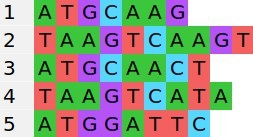
\includegraphics[width=0.15\textwidth]{images/s8}
	\caption{Conjunto de secuencias de la base de datos S8. Se utilizo Mega para colorear cada base.}
	\label{fig:s8}
\end{figure}




\subsection{Parametros}

Los parametros son descritos en la Tabla \ref{tab:param}. Para reducir el tiempo de procesamiento reducimos el valor de algunos parametros como la cantidad de iteraciones, el autor proponia en este caso 1000 iteraciones. Luego la cantidad de veces que se replico cada experimento era de 30 y nosotros solo lo replicamos 10 veces.

\begin{table}[h]
	\centering
	\caption{Parametros utilizados en los experimentos. Algunos parametros fueron distintos a los planteados por \cite{zablocki2009multiple} (iteraciones), con el objetivo de reducir el tiempo de procesamiento.}
	\begin{tabular}{p{4cm}p{1cm}}
		
		\textbf{Parametro} & \textbf{Valor} \\
		\hline			
		Iteraciones	& 30		\\				
		Cantidad de partículas & 25 \\
		Probabilidad de mutación & 0.2 \\ 
		\textit{Gaps} permitidos & 30\% \\	
		Cantidad de veces que se replico el experimento & 10 \\		
		\hline 
	\end{tabular}		
	\label{tab:param}
\end{table}

\section{Resultados}

En la Tabla \ref{tab:result}, se muestra el \textit{score} (resultado de la función objetivo) obtenido en cada base de datos. Como se puede apreciar, el \textit{score} depende de la complejidad del problema, por ejemplo en el conjunto de secuencias S8 obtenemos un score bajo, pero para las secuencias de S6 (la mas compleja), obtenemos un \textit{score} mucho mas grande. La idea es que mientras mayor sea el \textit{score}, es mejor. \\

\begin{table}[h]
	\centering
	\caption{Resultados obtenidos en cada base de datos. Se hicieron pruebas incluyendo y excluyendo la mutación.}
	\begin{tabular}{p{1cm}p{1.5cm}p{1.5cm}p{1cm}}
		
		\textbf{\textit{Dataset}} & \textbf{\textit{PSO} con mutación}  & \textbf{\textit{PSO} sin mutación} & \textbf{CLUSTALW} \\
		\hline			
		S6	& 12678	& 10012	& 18045 \\				
		S7 & 11105 & 9054 & 12564 \\
		S8 & 32 & 28 & 49 \\ 				
		\hline 
	\end{tabular}		
	\label{tab:result}
\end{table}


Para visualizar mejor el resultado de los alineamientos se utilizo la herramieta Mega, esta herramienta colorea cada base según su posición para ver mejor su alineamiento. En la Figura \ref{fig:s8_align}, mostramos el resultado luego de alinear el conjunto de secuencias de S8 utilizando PSO y CLUSTALW. Como podemos ver, existen muchas soluciones para cada problema, e incluso podemos llegar a tener un diferentes soluciones con un mismo \textit{score}. En la Figura \ref{fig:s7_align}, mostramos un parte del alineamiento de las secuencias de S7, recordemos que estas secuencias tienen una longitud de 457 bases.


\begin{figure}[h]
	\centering
	\begin{multicols}{2}
		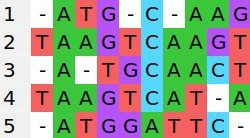
\includegraphics[width=0.15\textwidth]{images/s8_align}\par 
		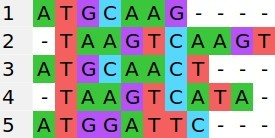
\includegraphics[width=0.17\textwidth]{images/s8_align_mega}\par 
	\end{multicols}
	\caption{\textbf{Izquierda}: Resultado luego de alinear las secuencias de la base de datos S8 utilizando PSO.\\  \textbf{Derecha}: Resultado luego de alinear las secuencias de la base de datos S8 utilizando CLUSTALW.}
	\label{fig:s8_align}
\end{figure}

\begin{figure}[!hbt]
	\centering
	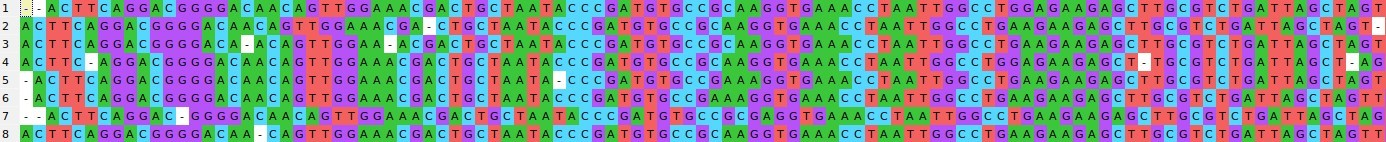
\includegraphics[width=0.47\textwidth]{images/s7_align}
	\caption{Resultado luego de alinear las secuencias de la base de datos S7 utilizando PSO. Solo se esta mostrando un extracto, porque las secuencias tienen una longitud de 457 bases.}
	\label{fig:s7_align}
\end{figure}


\section{Discusión}

De la Tabla \ref{tab:result}, comprobamos que el desempeño de PSO es bueno y casi llega a una solución similar a CLUSTAW. Además, uno de los problemas de PSO es que llega muy pronto a optimos locales, debido a eso, la versión de PSO con mutación tiene mejores resultados. Otro problema  de PSO y otros algoritmos similares, es la forma de definir el desplazamiento de cada partícula, en este trabajo se planteo utilizar un \textit{crossover}, pero existen trabajos recientes propuestos por \cite{zhan2019probpfp}, \cite{lalwani2019multi} y \cite{moustafa2017fragmented} donde obtienen mejores resultados modificando la función de movimiento de cada partícula y combinando PSO con las cadenas de Markov. \\

Una prueba visual del buen desempeño de PSO es presentado en las Figuras \ref{fig:s8_align} y \ref{fig:s7_align}. Como vemos en las imágenes, se aprecia que se ha obtenido un alineamiento aceptable. Cada base (letra) es representada con un color distinto y esta forma de visualización ayuda bastante para determinar el alineamiento entre dos o mas secuencias.

\section{Conclusiones}

La tesis propone el uso de PSO para solucionar el problema de MSA. El autor evalua los resultados en 8 bases de datos, que representan un conjunto de secuencias de diferentes longitudes. El autor obtuvo dichas secuencias de NCBI, pero al ser una tesis del 2009, algunas secuencias ya no estaban presentes.\\

El autor tambien propone aplicar una mutación a las partículas para evitar caer en optimos locales, esta mutación se basaba en insertar un \textit{gap} dentro de una secuencia de una partícula. Esta diversificación (mutación) mejoro el desempeño de PSO. \\

Para comprobar el desempeño de PSO, se comparó sus resultados con CLUSTALW. El desempeño de PSO fue bueno y logro un \textit{score} similar a CLUSTALW. En la actualidad existen varias modificaciones en la forma de como se define una partícula y la función de movimientno de esta con muy buenos resultados. \\


%\blinddocument

%A supplementary material section will always appear before the Reference list. If you're certain that your %submission won't have any supplementary material, you can add the \texttt{nosupp} option to the document %class declaration, i.e. 
%\begin{quote}
%\verb|\documentclass[nosupp]{cup-pan}|
%\end{quote}

%\clearpage

\bibliography{refs} 
\bibliographystyle{ieeetr}

\end{document}
